
\chapter{打破思维定式}

法国生物学家贝尔纳说过:妨碍学习的最大障碍,并不是未知的东西,而是已知的东西。其实他讲的就是思维定式的问题。
对于想提高记忆力和思维能力的人来说,一旦形成某种固有的思维定式,那就会极大地影响提升的效果。

\section{一切从右脑开始}


因为左右脑分工的原理,在记忆力和思维能力训练课程中,我们就要把左脑的抽象思维记忆转化成右脑的形象思维记忆。
这样能增加我们记忆的容量。


\section{联想能力的三个要点}

一个人的联想能力与记忆力和思维能力有非常大的关联性。
如果一个人具有十分活跃的联想能力,那么他必定具有强大的记忆能力和思维能力。

在联想的过程中,有以下三个关键要点:
\begin{itemize}
\item 夸张夸大\\
  如果把夸张夸大用在记忆资料的过程中,就能在我们的大脑里产生深刻的印象。
  因为可以让记忆的东西或者资料等变得新颖独特、生动形象、奇特鲜明。
  即使是常人觉得最难记忆的材料,只要运用夸张夸大这一原则进行加工过后,都会产生鲜明的形象存储在我们的大脑里面,让人印象深刻。

  例如,蝌蚪、冰箱、沙发、熊猫、插座、花瓶、青菜、圆桌、垃圾桶这些词汇。
  如果就这样读一遍这些词汇,我相信你几乎很难在大脑里形成一个完整的印象,但运用夸张夸大的原则,你的大脑就会立刻作出反应。
  比如,蝌蚪:一群黑压压的蝌蚪在水里游来游去;
  冰箱:堆得像几层楼一样高的冰箱;
  沙发:一条街上堆着像小山一样高的沙发;
  熊猫:竹林里面全是吃竹叶的熊猫;
  插座:插座铺成的路;
  花瓶:花瓶“啪”的一声打碎了;
  青菜:你去菜园里面摘了一篮子青菜;
  圆桌:你躺在几十张圆桌上;
  垃圾桶:你用手去掏垃圾桶手 上沾满了很恶心的垃圾。

\item 生动鲜明\\
  我们的大脑喜欢动态的,讨厌静态的。
  生动鲜明的图画当然比呆板的文字更能吸引我们大脑的注意。

  比如背诵古文,根据的理解,在头脑中或者绘画出有情节的图画。
  至今还记得《劝学》中描述的求学辛苦的画面。

\item 诙谐有趣\\
  比如《道德经》第十八章的原文:
  \begin{tcolorbox}
    大道废,有仁义; 智慧出,有大伪; 六亲不和,有孝慈; 国家昏乱,有忠臣。
  \end{tcolorbox}
  大刀废了(大道废),有人医(有仁义); 智慧很粗(智慧出),有大尾巴(有大伪); 六个亲戚都不和睦(六亲不和),有药吃(有孝慈); 国家很昏乱(国家昏乱),有忠臣。
\end{itemize}

\section{发散思维}

发散思维是不依常规,寻求变异,对给出的材料和信息从不同角度、向不同方向、用不同方法或途径进行分析和解决问题的一种思维方式,是一种非常重要的创造性思维。
在我们的生活和学习中,经常进行发散思维能力训练,就可以让我们的思维变得流畅、多端、灵活、新颖和精细,从而更大程度地提升我们的创造性。

有一道智力测验题:“用什么方法能使冰最快地变成水?”一般人往往回答要用加热、太阳晒等方法,但如果用发散思维,答案却是“去 掉‘冰’字偏旁两点,就变成水了”。
这就打破了人们的思维定式,拓宽人们的想象了。

如何训练自己的发散能力呢?
\begin{itemize}
\item 培养自己的观察力\\
  观察力可以把需要记忆的材料用右脑思维深深地储存在我们大脑里面。
  大脑对材料储存的细节越多、越仔细,说明观察的能力越强,在记忆的时候发散思维的能力就越强。

  在生活中,随时随地都有机会进行增强观察力的练习,以下的“场景再现”训练法是非常有效的:
  \begin{itemize}
  \item 走在街道、公园或者旅游景点时,我们可以边走边说出周围的 花草树木、颜色、方位。
  \item 看看身边匆匆而过的行人,当他从自己视线里消失后立刻回想 他的衣服、裤子、鞋帽的款式、颜色,身高、胖瘦以及身体最明显的特征等。
  \item 经过商场时,迅速把货架上的商品扫视一遍,等走出商场后, 仔细回忆货架上的每一件物品,越多越好,越仔细越好。
  \item 如果你实在不愿意出门,那你可以在电脑上玩一款游戏——大家来找茬,这对培养自己的观察力和视觉分辨能力是非常有帮助。
  \item 当你读完一篇文章后,试着把读到的情节用自己的语言将其中的场景复述出来。
  \item 看到电视新闻或者网上对人有启发的故事尽可能地用场景描述的方式讲给朋友或者身边的人听。
  \item 看完一部电影或者一集电视连续剧后,不妨把里面的场景尽可能详尽地讲给身边的人听。
  \end{itemize}
\item 激发自己的想象力\\
  如果一个人拥有十分丰富和活跃的想象力,他一定具备强大的记忆力,因为良好的记忆力与强大的想象力紧密相连。

  就记忆力和思维能力提升训练来讲,在进行想象力训练的时候无须让自己的想象符合逻辑,也不必担心自己的想象过于大胆,只需要把想象中的形象清清楚楚地刻画在脑海里,尽可能地把想象中的图像、动作、旋律等与不同的事物有效联系起来就好。

  集中想象力训练的具体方法:
  \begin{itemize}
  \item 梦境想象法\\
    在脑海里回忆自己的梦境,不管是美梦还是噩梦都可以。
    按以下的线索进行回忆:梦是彩色的吗?
    在哪里发生的?
    有哪些人?
    当时发生了什么事情?
    你的心情如何?
    假如你对所做的梦已经模糊了,那就请你做个白日梦吧,天马行空,任意发挥,将白日梦发挥到极致。
  \item 读图想象法\\
    对你生活或者工作当中遇到的每一幅图片,从以下步骤开始想象:
    从这张图中,你看到了什么?
    这张图这样做是为什么?
    如果图片上有人或者动物,请在自己的脑海中想象:
    这些人是谁?
    他们在干什么?
    这是在哪里?
    是什么时候呢?
    发生了什么事情?
    你还能想象到什么样的情景?
    请仔细看图,充分挖掘图片里的信息,然后闭目想象,越生动越好。
  \item 物体想象法\\
    请把生活中任意两样或三样东西随意组合在一起,试试看能创造出什么新东西呢?
    发挥你的想象力吧,任何东西都可以放在一起的。
    请在大脑里想象这个新东西是什么样子的,会有什么样的新功能呢?
    这种新功能能给我们带来什么样的改变呢?
  \item 听觉想象法\\
    听一首你喜欢的歌或者一篇有声散文,带着感情反复听几次,把自己投入音乐或者散文当中去。
    然后关掉声音,闭上眼睛回想。让动听的曲调或者散文的内容在你的脑海中回荡......
  \item 嗅觉想象法\\
    请找来一个水果,闻一闻水果的香气,再用小刀把水果切成两半,用鼻子深深地闻一闻,感受一下水果切开后的味道, 然后张开嘴咬一口。
    这时候,请闭上眼睛,体会嘴里面水果的味道和水果香味弥漫全身的感觉。
  \item 词句想象法\\
    词句想象法就是利用右脑的创造力把一些随机写出来的词语或者句子用图像串联起来,成为一幅生动有趣的场景。
    例如 我们随机写了这些词语:鞋子、布娃娃、冰箱、沙发、苹果、猪八戒、鼻子、铅笔、太阳、洗衣机。
    运用词句想象法串联起来就是:一双漂亮的鞋子被布娃娃塞进了冰箱里后,却发现沙发上的苹果被猪八戒用鼻子顶住,铅笔砸坏了太阳下的洗衣机。
    这样一串联就把一些毫无规律的词语演绎成了一幅有趣的场景。
  \end{itemize}
  
\end{itemize}

\section{注意力}

保持良好的注意力,是快速提升记忆力的关键条件。
在学习的过程中,注意力会让大脑迅速接收学习资料所发出来的信号,这个信号能迅速触动脑波激发我们的记忆潜能,注意力越集中,激发的大脑记忆潜能就越强大,记忆学习资料越轻松,速度就越快,学到的知识就越多。

注意力不集中的原因主要分外因和内因两类:外因和内因。

外因:就是外部对个体形成的干扰,比如噪声、对话、不舒服的椅子和桌子、不合适的灯光、电视、工作、家务、网络、电子邮件等。

内因:主要是个体自身的因素。比如饿了,累了,病了;对所做的事情没有动力,感到厌烦,没有兴趣;对环境焦虑,无法面对学习和工作的压力和烦恼;还有就是对自己或者环境的一些消极想法以及一些不切实际的白日梦等。


几种注意力训练的方法:
\begin{itemize}
\item 固点凝视法\\
  固点凝视法能让我们的视觉集中能力最大限度发挥出来,从而最大限度地增强我们的注意力。
  \begin{enumerate}
  \item 找一张无折痕的白纸,在上涂画一个0.5cm的圆点。
  \item 放轻松,自由呼吸,两眼睁大,双手举起白纸和眼睛平行,让黑点和眼睛相隔30cm左右。
  \item 凝视白纸上的黑点2分钟,尽量不要眨眼睛。
  \item 时间到了以后,两眼迅速望向白色的墙壁,看看墙壁上是否会出现一个白色的圆点,如果出现,让白色的圆点在墙壁上保持的时间越长越好。
    如果没有出现白色的圆点或者出现的时间只有短短几秒钟的话,请你务必每天坚持重复以上的步骤进行训练。
  \item 每天早、中、晚各训练一次,大约经过一周的训练后,你就能把白色的圆点保持3~4分钟,这时候,你的注意力就有了很大的提升,如果希望效果更好,继续坚持练习就好。
  \end{enumerate}
\item 静坐冥想法\\
  所谓静坐冥想法,就是在意识十分清醒的状态下停止意识对外的一切活动,达到“忘我”的一种快速提升注意力的心灵净化体操。
  通过静坐冥想强化自己对注意力的控制是优化和重塑大脑的最佳方法。

  \begin{enumerate}
  \item 选一个让自己舒服的姿势坐好。
  \item 挺直脊背,可以想象自己的头被一根绑在天花板上的绳子吊着。
  \item 闭上双眼,用鼻子深深且缓慢地吸气,让肺部充满空气,腹部和整个胸腔因而扩张,屏息4秒钟或更久,让自己享受这种吸入新鲜空气的感觉,然后用鼻子或嘴缓缓呼气,到接近呼完就把腹肌收缩,将腹 部所有气体排空。当你吐气时,感觉你释放出所有的忧虑、挂念、紧绷的情绪和压力。
  \item 冥想自己心灵深处有一汪蓝色的湖泊,湖泊平静得没有一丝涟漪。
    湖泊岸边,长满了花草树木,花草树木的影子倒映在湖泊里,色彩斑斓,十分清晰。
    然后再想象一朵朵美丽的牡丹花的影子在心灵湖泊上倒映出来,粉红的花瓣、细嫩的花蕊上点缀着金黄色的花粉。
    想得越逼真、越细致,心情便越沉静,注意力就会越来越好。
    也可以试着把周围的声音和冥想结合起来,如倾听到钟表嘀嗒嘀嗒的声音,可以把这声音想成雨水滴在心灵湖泊上所发出的声音,每滴一下,湖泊上便溅起一丝涟漪。
    你还可以一边倾听,一边数着这雨滴的数量,1,2,3,4,5......
    当数到100多次的时候,睁开双眼,你会觉得心情异常平静,通体舒畅,注意力特别集中。
  \item 每天这样冥想2次,每次2、3分钟,能有效控制精神涣散,收拢浮躁的心。
  \end{enumerate}
\item 舒尔特方格法\\
  如图\ref{fig:schulte-grid}所示。
  测试时,要求被测者用手指按1~25的顺序依次指出其位置,同时诵读出声,施测者在一旁记录所用时间,数完方格中25个数字所用时间越短,注意力水平越高。

  舒尔特方格的练习法:
  \begin{enumerate}
  \item 保持腹式呼吸,眼睛距离表格30~35cm,视点自然放在表的中心。
  \item 在所有字符全部清晰入目的前提下,按顺序找到1~25,注意不要顾此失彼,因找 一个字符而对其他字符视而不见。
  \item 每看完一个表,眼睛稍做休息,或闭目,或做眼保健操,不要过分疲劳,以免给眼睛带来损伤。
  \item 练习初期不考虑记忆因素,每天看10个表就好,循序渐进地增加难度。
  \end{enumerate}
\end{itemize}

\begin{figure}[!htbp]
  \centering
  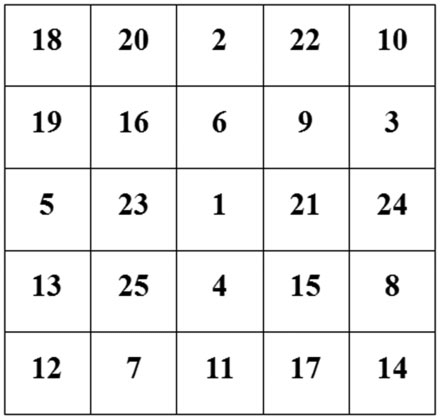
\includegraphics[width=0.6\textwidth]{schulte-grid}
  \caption{舒尔特25格表}
  \label{fig:schulte-grid}
\end{figure}


\section{构建联想能力的三种模式}

当一个人的五感受到外部信息的刺激时,大脑就会运用联结、转结和跳跃这三种模式同时将已知的信息和外部的信息进行有效的碰撞和对接,这种碰撞和对接会让我们的视野变得开阔,由此产生一些创造性的信息。


以“玫瑰花”为例,对“玫瑰花”进行联结,转结和跳跃这三种模式的联想:

联结:月季花,牡丹花,荷花,菊花,黄花,油菜花,食人花......

转结:花农,花棚,花车,商场,花店,土地,花茶,婚礼,超市,刀子,服装......

跳跃:金钱,跑车,航天飞机,死亡,中奖,奴隶,洗澡,房子,香水,昆虫......

对事物的联结其实就是通过对玫瑰花进行线性的联想,所有联想的东西都是跟玫瑰花同一个种类。
没有超出“花”这一物种的层面。
因为是线性的联想,人们总是习惯性地把相同类别的物体直接联系在一起。
这种线性的联结其实也有它的好处,但是要提升记忆力和思维能力,我们就必须尝试着摆脱这种线性联结方式,只有这样才能让联想更加自由。

转结是对玫瑰花进行纵向的联想。
虽然是纵向的思维,但是它们之间还是有紧密的关联性。这种转结的联想,提升了联想的宽度,让联想更加开阔。

至于跳跃,这个时候的思维就变得无拘无束。
我们可以横向、纵向天马行空地想象,不再受到逻辑的限制。
这种跳跃的联想跟玫瑰花看似没有任何关联,但它们之间其实是可以找到联系的。
任何两个概念经过四五个阶段就可以建立联想。
一个人在情人节那天靠卖玫瑰花赚取了很多金钱。
一个美女用玫瑰花装点自己的超级跑车。
宇航局给每一个在航天飞机的宇航员送了一支玫瑰花。
一个人吻了一下玫瑰花后就被毒死了。
一个男生买玫瑰花,店主送了他一张彩票,因为这张彩票,男生中 了500万元大奖。
奴隶因为一朵玫瑰花被奴隶主给残忍地杀害了。
花匠端来一盆水给玫瑰花洗澡。
房子的四周栽种着粉红色的玫瑰花。
香水大师用玫瑰花做成了一瓶香水。
一群又一群的昆虫飞过来停留在玫瑰花上。

\section{提升联想能力的三种方法}

\begin{itemize}
\item 联想开花训练\\
  就是以自己熟知的某 一个事物或者词组为“中心主题”展开联想,发展思维,所发散的主题内容不受任何限制地向四面八方发射,就像一朵绽开的花,花瓣向四周展开一样。
\item 联想接龙训练\\
  就是首先选定好某 一个事物或者词或者词组为“中心主题”,然后由中心主题激发出一个联想,再由激发出的联想变成主题继续激发出下一个联想,像条长龙一样无限制地往下延伸。
\item 太极八卦训练\\
  太极生两仪,两仪生四象,四象生八卦。

  以手机为例,手机为太极,太极生两仪,阴阳正负等。
  手机原本的功能,或者说目的是为阳,阴为不是手机原本带有的功能可是做的事。
  比如手机可以通讯,看视频,照明,导航等等,阴则为,手机可以砸人,手机可以垫桌子,手机可以做砝码等等。
  四象,是为生老病死,东南西北,春夏秋冬,金木水火等,
  新手机,旧手机,有毛病的手机,坏了的手机可以做什么呢?
  八卦则近一步扩展。
\end{itemize}


\section{记忆}

\argument{注意联想}和\argument{发散}。

\argument{联想}要\argument{夸张生动有趣},用\argument{开花,接龙}和\argument{八卦}提升。
\begin{figure}[H]
  \centering
  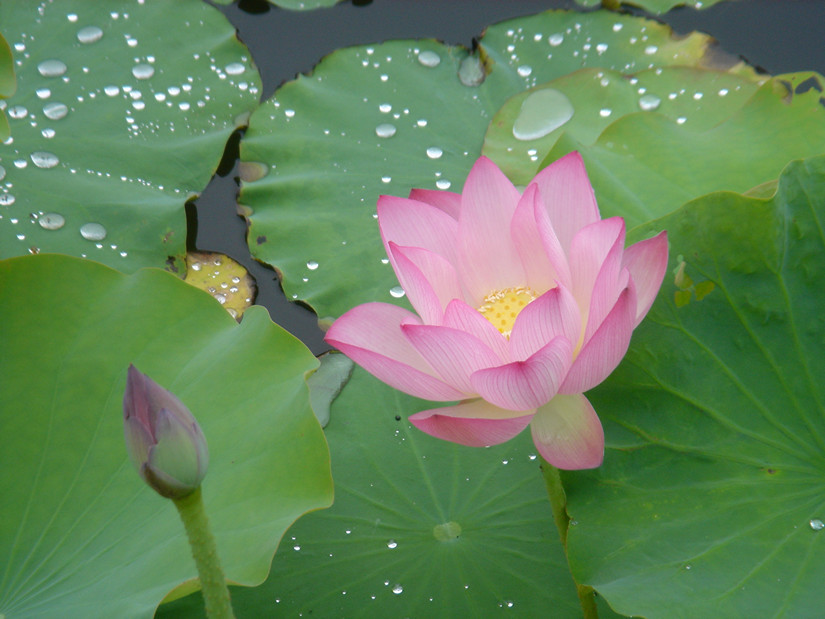
\includegraphics[width=0.3\textwidth]{flower}
  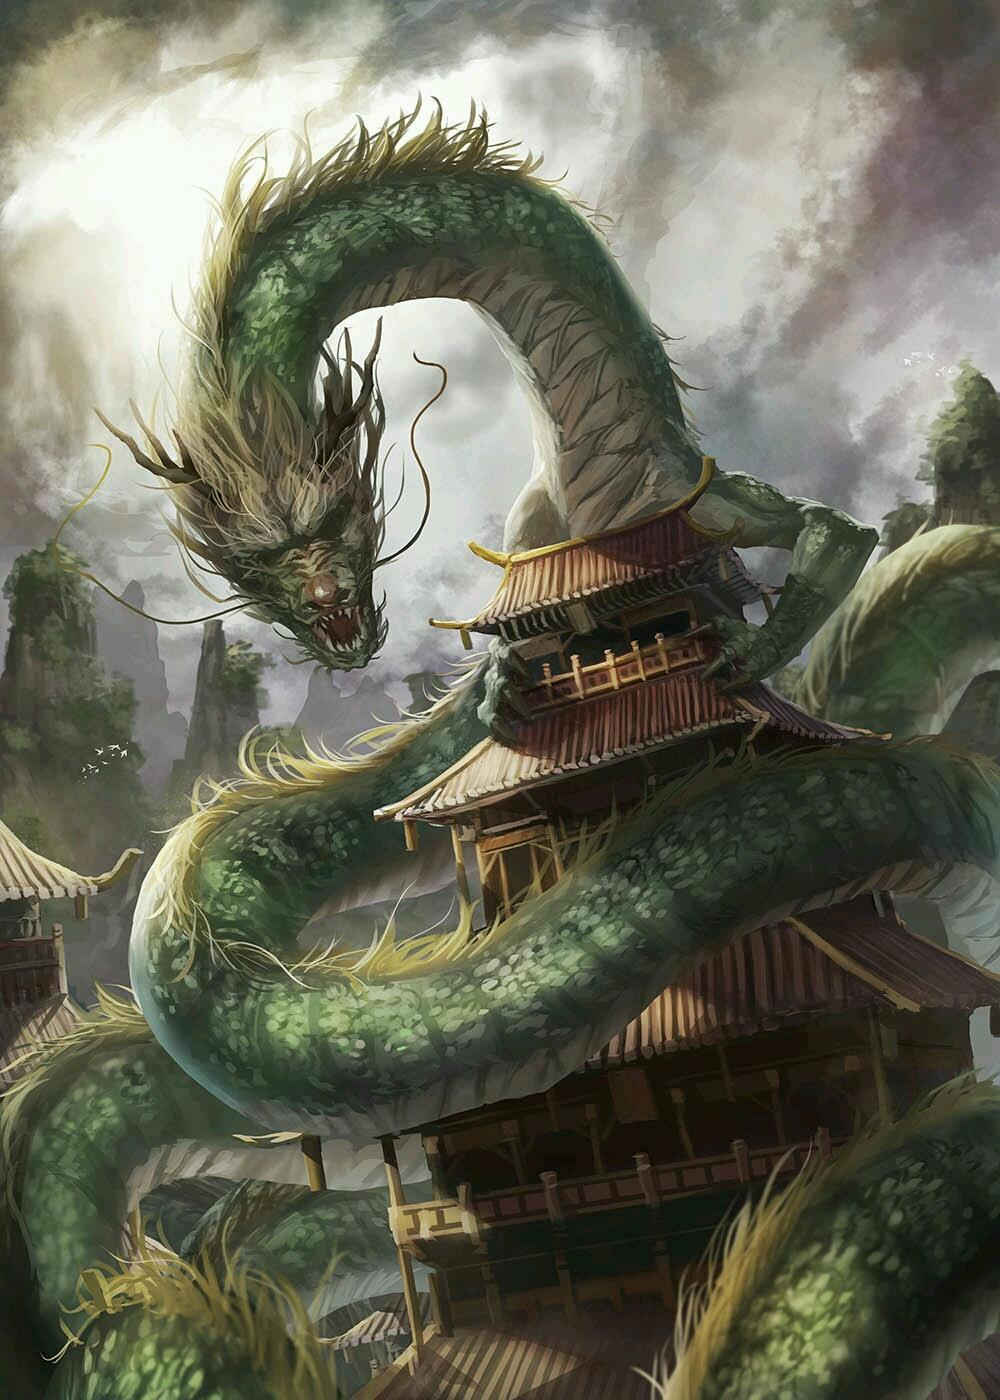
\includegraphics[width=0.3\textwidth]{dragon}
  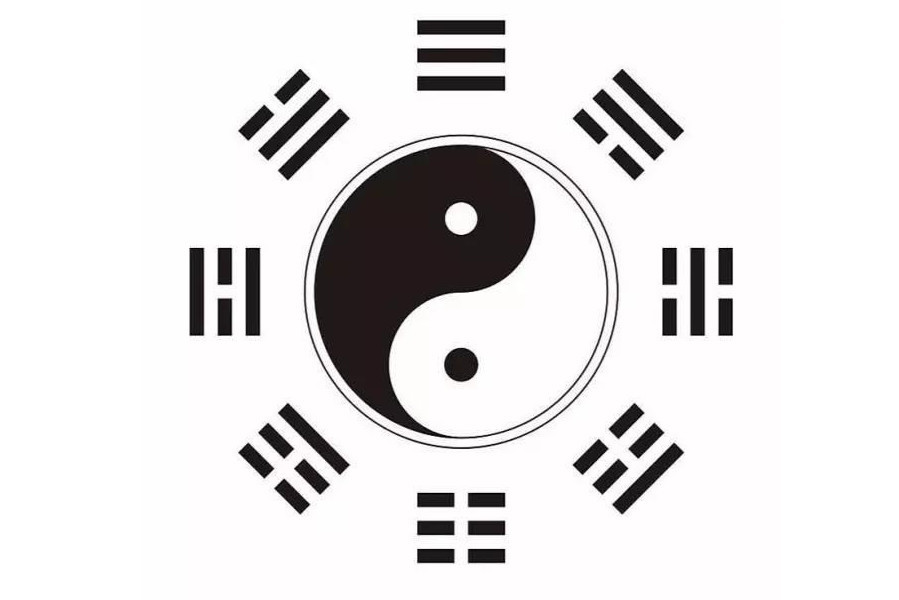
\includegraphics[width=0.3\textwidth]{bagua}  
\end{figure}
\argument{发散}与\argument{观察}和\argument{想象}相关。

注意力训练:固点,冥想,舒尔特。

\begin{figure}[H]
  \centering
  
\includegraphics[width=0.3\textwidth]{dot}
  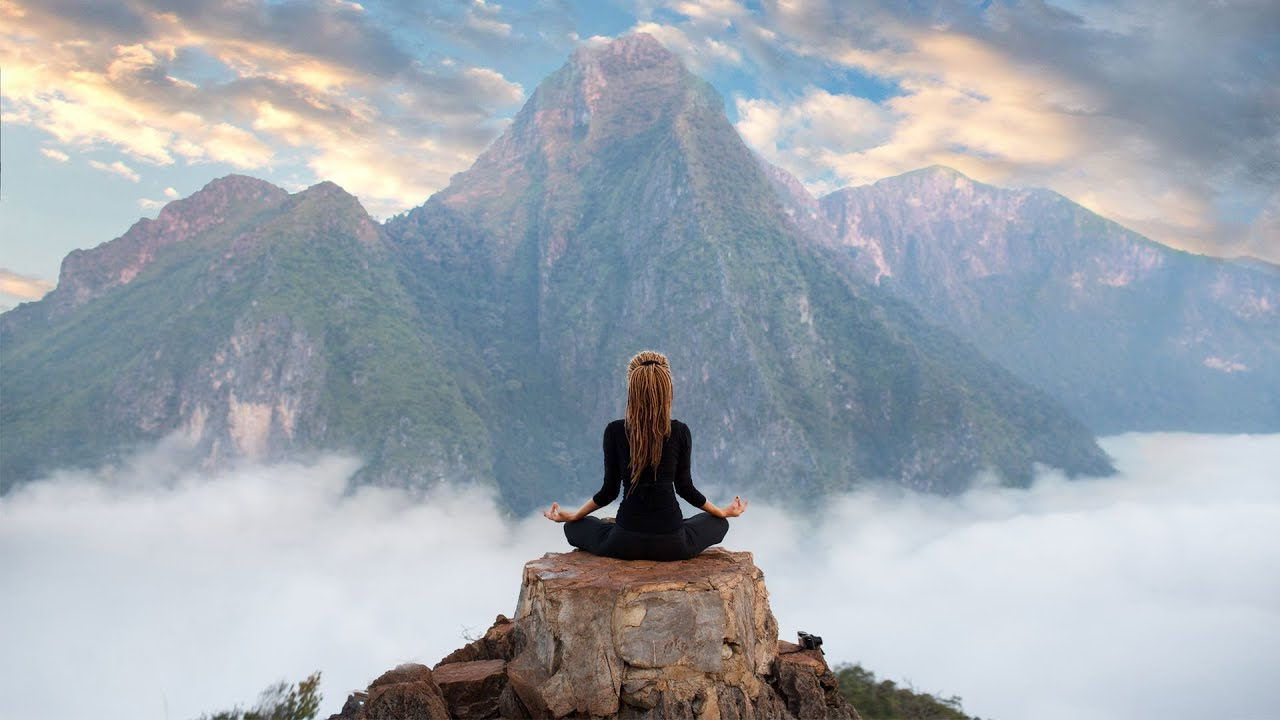
\includegraphics[width=0.3\textwidth]{meditation}
  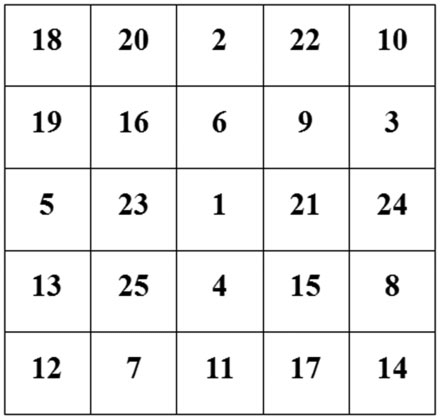
\includegraphics[width=0.3\textwidth]{schulte-grid}  
\end{figure}


\begin{tcolorbox}
  每天只吃土豆,放屁放的\argument{腚湿}了,
  \argument{联想}出\argument{主意(注意)} 给员工\argument{发膳(发散)}。
  为了\argument{提升联想}销量,张生动建议把logo改成\argument{华(开花)龙(接龙)}盘\argument{太极}。
  联想\argument{夸张生动}的logo\argument{有趣}。
  而张生动坐在\argument{竹椅里(注意力)}想\argument{寻找初恋(训练)}的感觉,有\argument{点(固点)}\argument{想(冥想)}\argument{放歌(舒尔特方格)}。
  联想要\argument{构建}\argument{廉洁(联结)}的工作环境,张生动却私自\argument{转借(转结)}了公款给初恋,最后\argument{跳跃}到其他公司了。
\end{tcolorbox}

%%% Local Variables:
%%% mode: latex
%%% TeX-master: "memory"
%%% End:
